% Archivo de caracterización de infraestructura corregido

% Torre HP 1
\begin{table}[H]
\centering
\scriptsize % Tamaño de fuente más pequeño
\setlength{\tabcolsep}{2pt} % Menor espacio entre columnas
\renewcommand{\arraystretch}{1.0} % Espaciado más ajustado
\caption{Ficha técnica --- Torre 1}\label{tab:torre-hp-1}
\begin{tabular}{|p{0.5\textwidth}|p{0.2\textwidth}|} % Columnas más estrechas
\hline
\multicolumn{2}{|l|}{\textbf{DESCRIPCIÓN FÍSICA:} Servidor tipo torre} \\ \hline
\textbf{TIPO DE RECURSO:} Torre &
\multirow{5}{*}{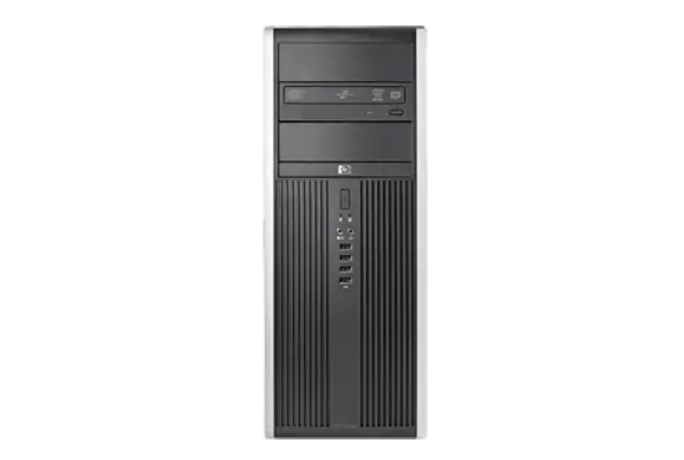
\includegraphics[width=0.18\textwidth,keepaspectratio]{tablas-images/cp1/torres/torre-1.png}} \\ \cline{1-1}
\textbf{MODELO:} Desconocido & \\ \cline{1-1}
\textbf{MARCA:} HP & \\ \cline{1-1}
\textbf{CÓDIGO DE INVENTARIO:} 7 24390 49867 3 & \\ \cline{1-1}
\textbf{NÚMERO EN CPD:} 14 & \\ \hline
\multicolumn{2}{|l|}{\textbf{ESPECIFICACIONES TÉCNICAS}} \\ \hline
\multicolumn{2}{|p{0.7\textwidth}|}{ % Ancho ajustado
- 8 USB (4 frontal, 4 trasera)
- Audio y micrófono
- HDMI
- Lector DVD
- 3 Ethernet
- DisplayPort
- PS/2 (Teclado/Ratón)
} \\ \hline
\multicolumn{2}{|l|}{\textbf{PROPÓSITO:} Hipervisor XCP-ng} \\ \hline
\multicolumn{2}{|l|}{\textbf{OPORTUNIDAD DE USO:} Proyectos del \GRID} \\ \hline
\multicolumn{2}{|p{0.7\textwidth}|}{\textbf{OBSERVACIONES:} Sin modelo. Equipo adaptado para virtualización.} \\ \hline
\end{tabular}
\end{table}

% Torre 2
\begin{table}[H]
\centering
\scriptsize
\setlength{\tabcolsep}{2pt}
\renewcommand{\arraystretch}{1.0}
\caption{Ficha técnica --- Torre 2}\label{tab:torre-2}
\begin{tabular}{|p{0.5\textwidth}|p{0.2\textwidth}|}
\hline
\multicolumn{2}{|l|}{\textbf{DESCRIPCIÓN FÍSICA:} Servidor tipo torre} \\ \hline
\textbf{TIPO DE RECURSO:} Torre & 
\multirow{5}{*}{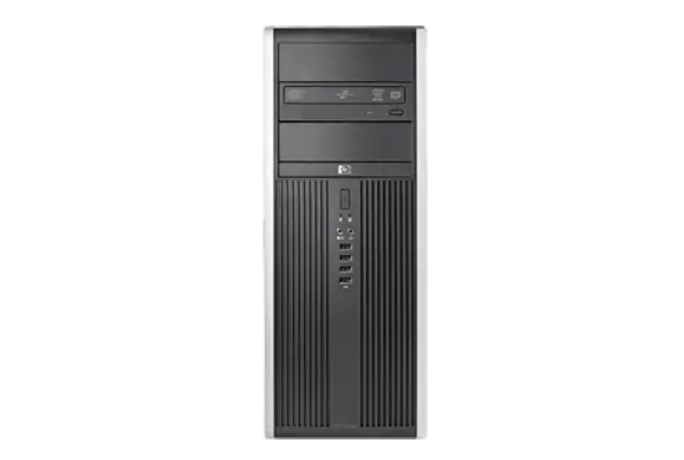
\includegraphics[width=0.18\textwidth,keepaspectratio]{tablas-images/cp1/torres/torre-1.png}} \\ \cline{1-1}
\textbf{MODELO:} Desconocido & \\ \cline{1-1}
\textbf{MARCA:} HP & \\ \cline{1-1}
\textbf{CÓDIGO DE INVENTARIO:} 7 24390 49861 1 & \\ \cline{1-1}
\textbf{NÚMERO EN CPD:} 12 & \\ \hline
\multicolumn{2}{|l|}{\textbf{ESPECIFICACIONES TÉCNICAS}} \\ \hline
\multicolumn{2}{|p{0.7\textwidth}|}{
- 8 USB (4 frontal, 4 trasera)
- Audio y micrófono
- HDMI
- Lector DVD
- 3 Ethernet
- DisplayPort
- PS/2 (Teclado/Ratón)
} \\ \hline
\multicolumn{2}{|l|}{\textbf{PROPÓSITO:} Hipervisor XCP-ng} \\ \hline
\multicolumn{2}{|l|}{\textbf{OPORTUNIDAD DE USO:} Proyectos del \GRID} \\ \hline
\multicolumn{2}{|p{0.7\textwidth}|}{\textbf{OBSERVACIONES:} Sin modelo. Equipo adaptado para virtualización.} \\ \hline
\end{tabular}
\end{table}

% Torre 3
\begin{table}[H]
\centering
\scriptsize
\setlength{\tabcolsep}{2pt}
\renewcommand{\arraystretch}{1.0}
\caption{Ficha técnica -- Torre 3}\label{tab:torre-3}
\begin{tabular}{|p{0.5\textwidth}|p{0.2\textwidth}|}
\hline
\multicolumn{2}{|l|}{\textbf{DESCRIPCIÓN FÍSICA:} Servidor tipo torre} \\ \hline
\textbf{TIPO DE RECURSO:} Torre & 
\multirow{5}{*}{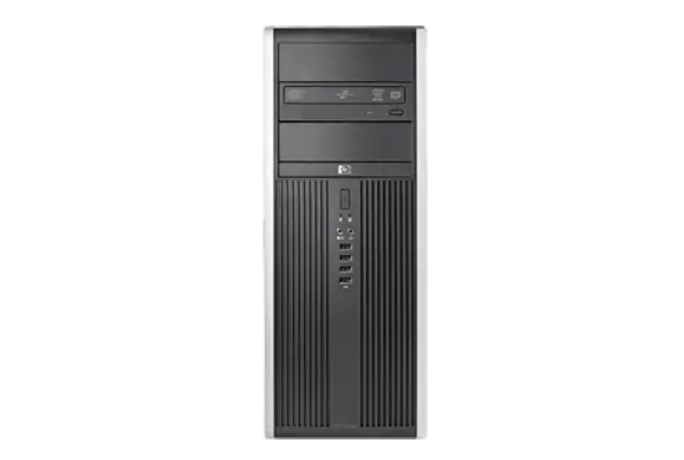
\includegraphics[width=0.18\textwidth,keepaspectratio]{tablas-images/cp1/torres/torre-1.png}} \\ \cline{1-1}
\textbf{MODELO:} Desconocido & \\ \cline{1-1}
\textbf{MARCA:} HP & \\ \cline{1-1}
\textbf{CÓDIGO DE INVENTARIO:} 7 24390 49969 4 & \\ \cline{1-1}
\textbf{NÚMERO EN CPD:} 13 & \\ \hline
\multicolumn{2}{|l|}{\textbf{ESPECIFICACIONES TÉCNICAS}} \\ \hline
\multicolumn{2}{|p{0.7\textwidth}|}{
- 8 USB (4 frontal, 4 trasera)
- Audio y micrófono
- HDMI
- Lector DVD
- 3 Ethernet
- DisplayPort
- PS/2 (Teclado/Ratón)
} \\ \hline
\multicolumn{2}{|l|}{\textbf{PROPÓSITO:} Hipervisor XCP-ng} \\ \hline
\multicolumn{2}{|l|}{\textbf{OPORTUNIDAD DE USO:} Proyectos del \GRID} \\ \hline
\multicolumn{2}{|p{0.7\textwidth}|}{\textbf{OBSERVACIONES:} Sin modelo. Equipo adaptado para virtualización.} \\ \hline
\end{tabular}
\end{table}

% Torre 4
\begin{table}[H]
\centering
\scriptsize
\setlength{\tabcolsep}{2pt}
\renewcommand{\arraystretch}{1.0}
\caption{Ficha técnica --- Torre 4}\label{tab:torre-4}
\begin{tabular}{|p{0.5\textwidth}|p{0.2\textwidth}|}
\hline
\multicolumn{2}{|l|}{\textbf{DESCRIPCIÓN FÍSICA:} Servidor tipo torre} \\ \hline
\textbf{TIPO DE RECURSO:} Torre & 
\multirow{5}{*}{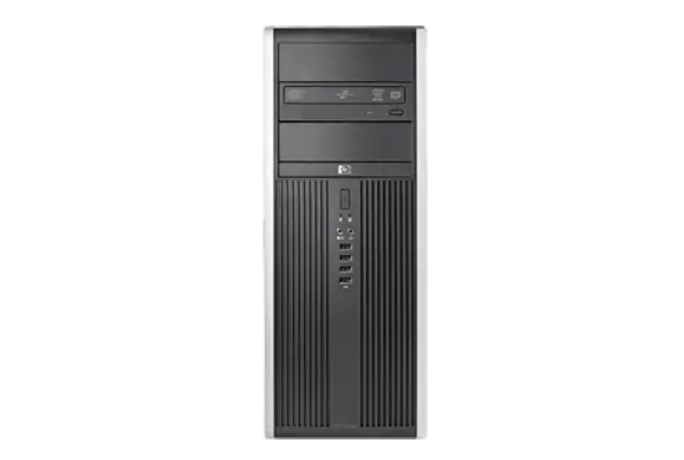
\includegraphics[width=0.18\textwidth,keepaspectratio]{tablas-images/cp1/torres/torre-1.png}} \\ \cline{1-1}
\textbf{MODELO:} Desconocido & \\ \cline{1-1}
\textbf{MARCA:} HP & \\ \cline{1-1}
\textbf{CÓDIGO DE INVENTARIO:} 7 24390 49879 4 & \\ \cline{1-1}
\textbf{NÚMERO EN CPD:} 14 & \\ \hline
\multicolumn{2}{|l|}{\textbf{ESPECIFICACIONES TÉCNICAS}} \\ \hline
\multicolumn{2}{|p{0.7\textwidth}|}{
- 8 USB (4 frontal, 4 trasera)
- Audio y micrófono
- HDMI
- Lector DVD
- 3 Ethernet
- DisplayPort
- PS/2 (Teclado/Ratón)
} \\ \hline
\multicolumn{2}{|l|}{\textbf{PROPÓSITO:} Hipervisor XCP-ng} \\ \hline
\multicolumn{2}{|l|}{\textbf{OPORTUNIDAD DE USO:} Proyectos del \GRID} \\ \hline
\multicolumn{2}{|p{0.7\textwidth}|}{\textbf{OBSERVACIONES:} Sin modelo. Equipo adaptado para virtualización.} \\ \hline
\end{tabular}
\end{table}


Los cuadros~\ref{tab:torre-5} y~\ref{tab:torre-6} detallan las características de dos servidores tipo torre HP, modelo G9, destinados a operar como hipervisores bajo XCP-ng. Ambos equipos, identificados en el inventario con los códigos 72992 y 72976 y ubicados en los puestos 22 y 21 del CPD, respectivamente, cuentan con especificaciones técnicas similares: nueve puertos USB (cuatro frontales y cinco posteriores), entradas y salidas de audio y micrófono, conexión HDMI, lector de DVD, una interfaz Ethernet, dos puertos DisplayPort y un procesador Intel vPro i9, lo que les otorga un mayor rendimiento frente a los servidores del mismo entorno. Estos equipos han sido adaptados para virtualización, reforzando la infraestructura tecnológica del GRID y ampliando las capacidades de cómputo necesarias para el desarrollo de entornos virtualizados de alto desempeño.
% Torre 5
\begin{table}[H]
\centering
\scriptsize
\setlength{\tabcolsep}{2pt}
\renewcommand{\arraystretch}{1.0}
\caption{Ficha técnica --- Torre 5}\label{tab:torre-5}
\begin{tabular}{|p{0.5\textwidth}|p{0.2\textwidth}|}
\hline
\multicolumn{2}{|l|}{\textbf{DESCRIPCIÓN FÍSICA:} Servidor tipo torre} \\ \hline
\textbf{TIPO DE RECURSO:} Torre & 
\multirow{5}{*}{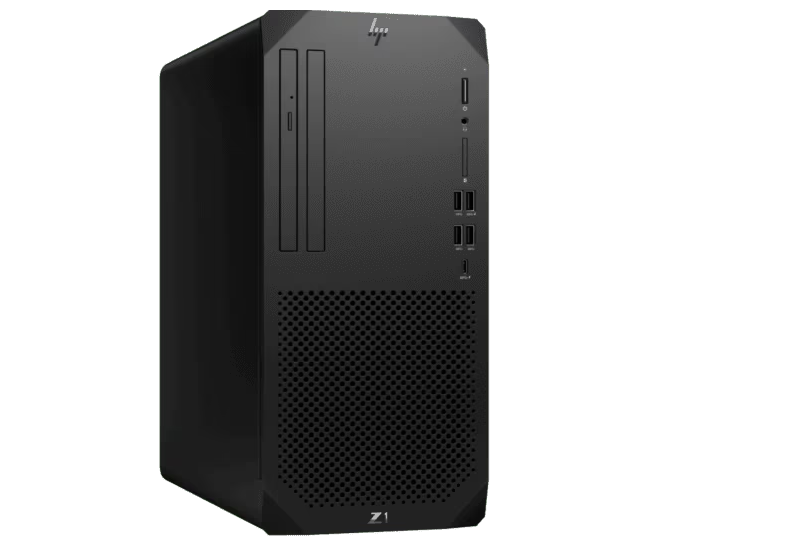
\includegraphics[width=0.18\textwidth,keepaspectratio]{tablas-images/cp1/torres/torre-2.png}} \\ \cline{1-1}
\textbf{MODELO:} G9 & \\ \cline{1-1}
\textbf{MARCA:} HP & \\ \cline{1-1}
\textbf{CÓDIGO DE INVENTARIO:} 72992 & \\ \cline{1-1}
\textbf{NÚMERO EN CPD:} 22 & \\ \hline
\multicolumn{2}{|l|}{\textbf{ESPECIFICACIONES TÉCNICAS}} \\ \hline
\multicolumn{2}{|p{0.7\textwidth}|}{
- 9 USB (4 frontal, 5 trasera)
- Audio y micrófono
- HDMI
- Lector DVD
- 1 Ethernet
- 2 DisplayPort
- Procesador Intel vPro i9
} \\ \hline
\multicolumn{2}{|l|}{\textbf{PROPÓSITO:} Hipervisor XCP-ng} \\ \hline
\multicolumn{2}{|l|}{\textbf{OPORTUNIDAD DE USO:} Proyectos del \GRID} \\ \hline
\multicolumn{2}{|p{0.7\textwidth}|}{\textbf{OBSERVACIONES:} Equipo adaptado para virtualización.} \\ \hline
\end{tabular}
\end{table}

% Torre 6
\begin{table}[H]
\centering
\scriptsize
\setlength{\tabcolsep}{2pt}
\renewcommand{\arraystretch}{1.0}
\caption{Ficha técnica --- Torre 6}
\label{tab:torre-6}
\begin{tabular}{|p{0.5\textwidth}|p{0.2\textwidth}|}
\hline
\multicolumn{2}{|l|}{\textbf{DESCRIPCIÓN FÍSICA:} Servidor tipo torre} \\ \hline
\textbf{TIPO DE RECURSO:} Torre & 
\multirow{5}{*}{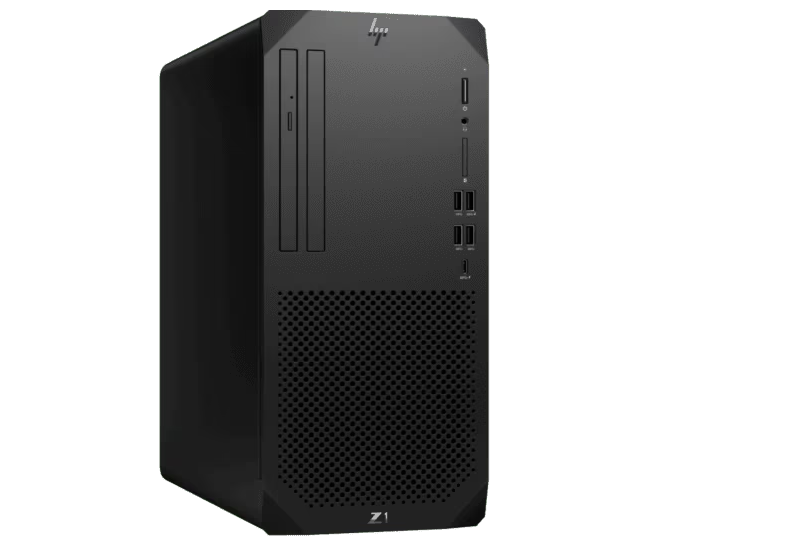
\includegraphics[width=0.18\textwidth,keepaspectratio]{tablas-images/cp1/torres/torre-2.png}} \\ \cline{1-1}
\textbf{MODELO:} G9 & \\ \cline{1-1}
\textbf{MARCA:} HP & \\ \cline{1-1}
\textbf{CÓDIGO DE INVENTARIO:} 72976 & \\ \cline{1-1}
\textbf{NÚMERO EN CPD:} 21 & \\ \hline
\multicolumn{2}{|l|}{\textbf{ESPECIFICACIONES TÉCNICAS}} \\ \hline
\multicolumn{2}{|p{0.7\textwidth}|}{
- 9 USB (4 frontal, 5 trasera)
- Audio y micrófono
- HDMI
- Lector DVD
- 1 Ethernet
- 2 DisplayPort
- Procesador Intel vPro i9
} \\ \hline
\multicolumn{2}{|l|}{\textbf{PROPÓSITO:} Hipervisor XCP-ng} \\ \hline
\multicolumn{2}{|l|}{\textbf{OPORTUNIDAD DE USO:} Proyectos del \GRID} \\ \hline
\multicolumn{2}{|p{0.7\textwidth}|}{\textbf{OBSERVACIONES:} Equipo adaptado para virtualización.} \\ \hline
\end{tabular}
\end{table}

El cuadro~\ref{tab:torre-7} presenta la ficha técnica del servidor tipo torre identificado como Torre 7, perteneciente a la marca Argom Tech y sin código de inventario asignado, ubicado en el puesto 11 del \CPD\. Este equipo dispone de un procesador Intel Pentium 62030 de 3.00 GHz con arquitectura x64, memoria RAM de 16 GB, disco duro de 1 TB, unidad de CD/DVD y tarjetas de video y sonido integradas. Su propósito principal es operar como hipervisor bajo la plataforma XCP-ng. Cabe destacar que en este servidor se encuentra implementada la solución arquitectónica propuesta, lo que lo convierte en un recurso fundamental para la validación y consolidación del entorno de contenedores diseñado para el \GRID.
% Torre 7
\begin{table}[H]
\centering
\scriptsize
\setlength{\tabcolsep}{2pt}
\renewcommand{\arraystretch}{1.0}
\caption{Ficha técnica --- Torre 7}\label{tab:torre-7}
\begin{tabular}{|p{0.5\textwidth}|p{0.2\textwidth}|}
\hline
\multicolumn{2}{|l|}{\textbf{DESCRIPCIÓN FÍSICA:} Servidor tipo torre} \\ \hline
\textbf{TIPO DE RECURSO:} Torre & 
\multirow{5}{*}{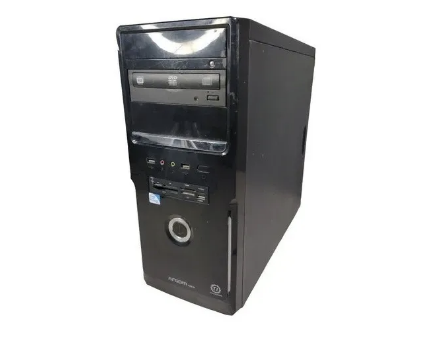
\includegraphics[width=0.18\textwidth,keepaspectratio]{tablas-images/cp1/torres/ATX.png}} \\ \cline{1-1}
\textbf{MODELO:} Argom tech & \\ \cline{1-1}
\textbf{MARCA:} Argom tech & \\ \cline{1-1}
\textbf{CÓDIGO DE INVENTARIO:} Sin código & \\ \cline{1-1}
\textbf{NÚMERO EN CPD:} 11 & \\ \hline
\multicolumn{2}{|l|}{\textbf{ESPECIFICACIONES TÉCNICAS}} \\ \hline
\multicolumn{2}{|p{0.7\textwidth}|}{
- Procesador: Intel Pentium 62030 3.00GHz
- Arquitectura: X64
- RAM: 16GB
- Disco: 1024GB
- Unidad CD/DVD: Sí
- Tarjeta video: Integrada
- Tarjeta sonido: Integrada
} \\ \hline
\multicolumn{2}{|l|}{\textbf{PROPÓSITO:} Hipervisor XCP-ng} \\ \hline
\multicolumn{2}{|l|}{\textbf{OPORTUNIDAD DE USO:} Proyectos del \GRID} \\ \hline
\multicolumn{2}{|p{0.7\textwidth}|}{\textbf{OBSERVACIONES:} Equipo adaptado para virtualización.} \\ \hline
\end{tabular}
\end{table}

Los cuadros~\ref{tab:rack-1} al~\ref{tab:rack-5} describen cinco servidores tipo rack, modelo System x3250 M4 de la marca IBM, los cuales  se ubican en el rack 1 del \CPD. Estos equipos, identificados con diferentes códigos dentro de la topología de red se ubica en los puestos 55, 54, 53 y 52. Presentan características técnicas homogéneas: procesador Intel Xeon E3\-1220v2, controlador SATA integrado, dos ranuras PCI Express, cuatro unidades SAS/SATA con capacidad de intercambio en caliente, fuente redundante de 460W, sistema de gestión integrado, cuatro puertos USB (dos frontales y dos posteriores) y lector de DVD.\@Su propósito principal es la prestación de servicios de cómputo y la provisión de recursos tecnológicos para estudiantes, además de la generación de máquinas virtuales orientadas a prácticas académicas.
% Rack 1
\begin{table}[H]
\centering
\scriptsize
\setlength{\tabcolsep}{2pt}
\renewcommand{\arraystretch}{1.0}
\caption{Ficha técnica --- Rack 1}\label{tab:rack-1}
\begin{tabular}{|p{0.5\textwidth}|p{0.2\textwidth}|}
\hline
\multicolumn{2}{|l|}{\textbf{DESCRIPCIÓN FÍSICA:} Servidor tipo rack} \\ \hline
\textbf{TIPO DE RECURSO:} Servidor & 
\multirow{5}{*}{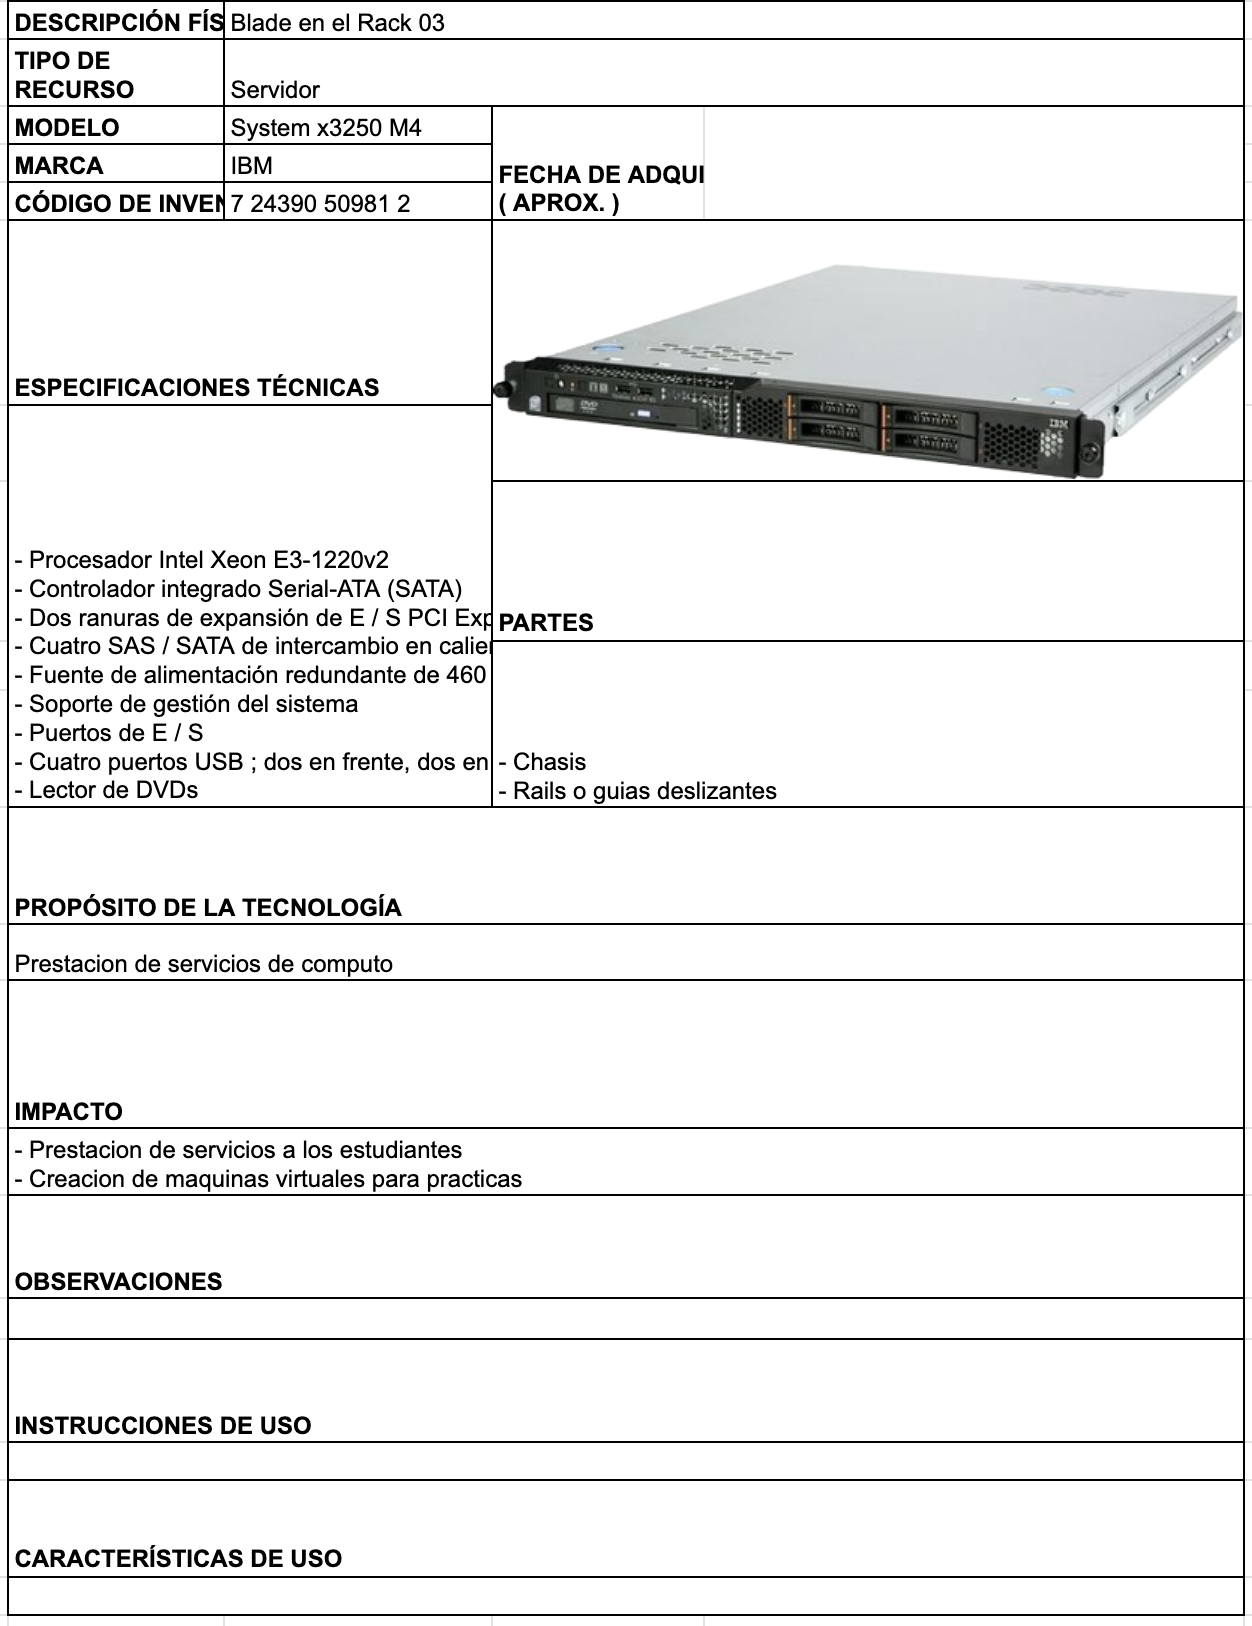
\includegraphics[width=0.18\textwidth,keepaspectratio]{tablas-images/cp1/racks/rack-1.png}} \\ \cline{1-1}
\textbf{MODELO:} System x3250 M4 & \\ \cline{1-1}
\textbf{MARCA:} IBM & \\ \cline{1-1}
\textbf{CÓDIGO DE INVENTARIO:} 7 24390 50981 & \\ \cline{1-1}
\textbf{NUMERO EN CPD:} 55 & \\ \hline
\multicolumn{2}{|l|}{\textbf{ESPECIFICACIONES TÉCNICAS}} \\ \hline
\multicolumn{2}{|p{0.7\textwidth}|}{
- Procesador Intel Xeon E3-1220v2
- Controlador SATA integrado
- 2 ranuras PCI Express
- 4 SAS/SATA intercambio en caliente
- Fuente redundante 460W
- Gestión del sistema
- 4 puertos USB (2 frontal, 2 trasero)
- Lector DVD
} \\ \hline
\multicolumn{2}{|l|}{\textbf{PROPÓSITO:} Prestación de servicios de cómputo} \\ \hline
\multicolumn{2}{|p{0.7\textwidth}|}{\textbf{IMPACTO:} 
- Servicios a estudiantes
- Máquinas virtuales para prácticas} \\ \hline
\multicolumn{2}{|p{0.7\textwidth}|}{\textbf{OBSERVACIONES:} Ninguna} \\ \hline
\end{tabular}
\end{table}

% Rack 2
\begin{table}[H]
\centering
\scriptsize
\setlength{\tabcolsep}{2pt}
\renewcommand{\arraystretch}{1.0}
\caption{Ficha técnica --- Rack 2}
\label{tab:rack-2}
\begin{tabular}{|p{0.5\textwidth}|p{0.2\textwidth}|}
\hline
\multicolumn{2}{|l|}{\textbf{DESCRIPCIÓN FÍSICA:} Servidor tipo rack} \\ \hline
\textbf{TIPO DE RECURSO:} Servidor & 
\multirow{5}{*}{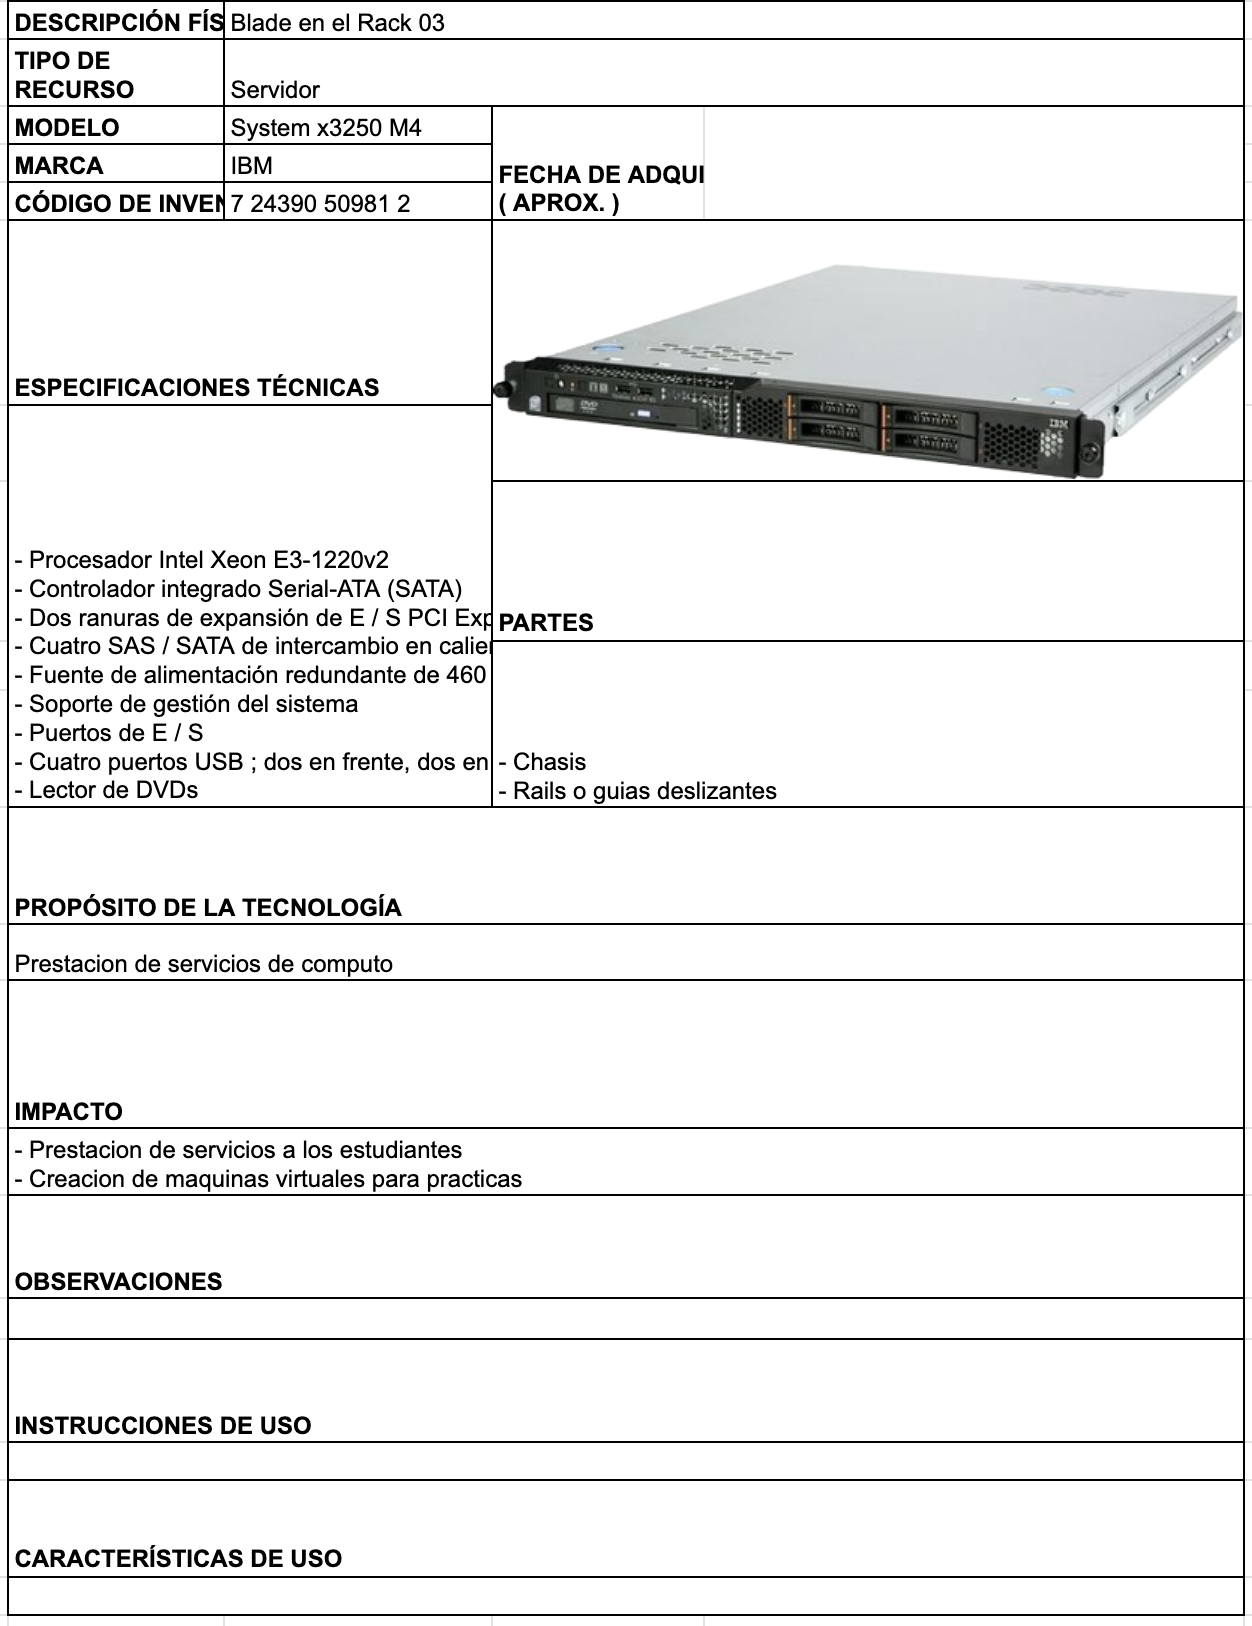
\includegraphics[width=0.18\textwidth,keepaspectratio]{tablas-images/cp1/racks/rack-1.png}} \\ \cline{1-1}
\textbf{MODELO:} System x3250 M4 & \\ \cline{1-1}
\textbf{MARCA:} IBM & \\ \cline{1-1}
\textbf{CÓDIGO DE INVENTARIO:} 7 24390 50980 & \\ \cline{1-1}
\textbf{NUMERO EN CPD:} 54 & \\ \hline
\multicolumn{2}{|l|}{\textbf{ESPECIFICACIONES TÉCNICAS}} \\ \hline
\multicolumn{2}{|p{0.7\textwidth}|}{
- Procesador Intel Xeon E3-1220v2
- Controlador SATA integrado
- 2 ranuras PCI Express
- 4 SAS/SATA intercambio en caliente
- Fuente redundante 460W
- Gestión del sistema
- 4 puertos USB (2 frontal, 2 trasero)
- Lector DVD
} \\ \hline
\multicolumn{2}{|l|}{\textbf{PROPÓSITO:} Prestación de servicios de cómputo} \\ \hline
\multicolumn{2}{|p{0.7\textwidth}|}{\textbf{IMPACTO:} 
- Servicios a estudiantes
- Máquinas virtuales para prácticas} \\ \hline
\multicolumn{2}{|p{0.7\textwidth}|}{\textbf{OBSERVACIONES:} Ninguna} \\ \hline
\end{tabular}
\end{table}

% Rack 3
\begin{table}[H]
\centering
\scriptsize
\setlength{\tabcolsep}{2pt}
\renewcommand{\arraystretch}{1.0}
\caption{Ficha técnica --- Rack 3}
\label{tab:rack-3}
\begin{tabular}{|p{0.5\textwidth}|p{0.2\textwidth}|}
\hline
\multicolumn{2}{|l|}{\textbf{DESCRIPCIÓN FÍSICA:} Servidor tipo rack} \\ \hline
\textbf{TIPO DE RECURSO:} Servidor & 
\multirow{5}{*}{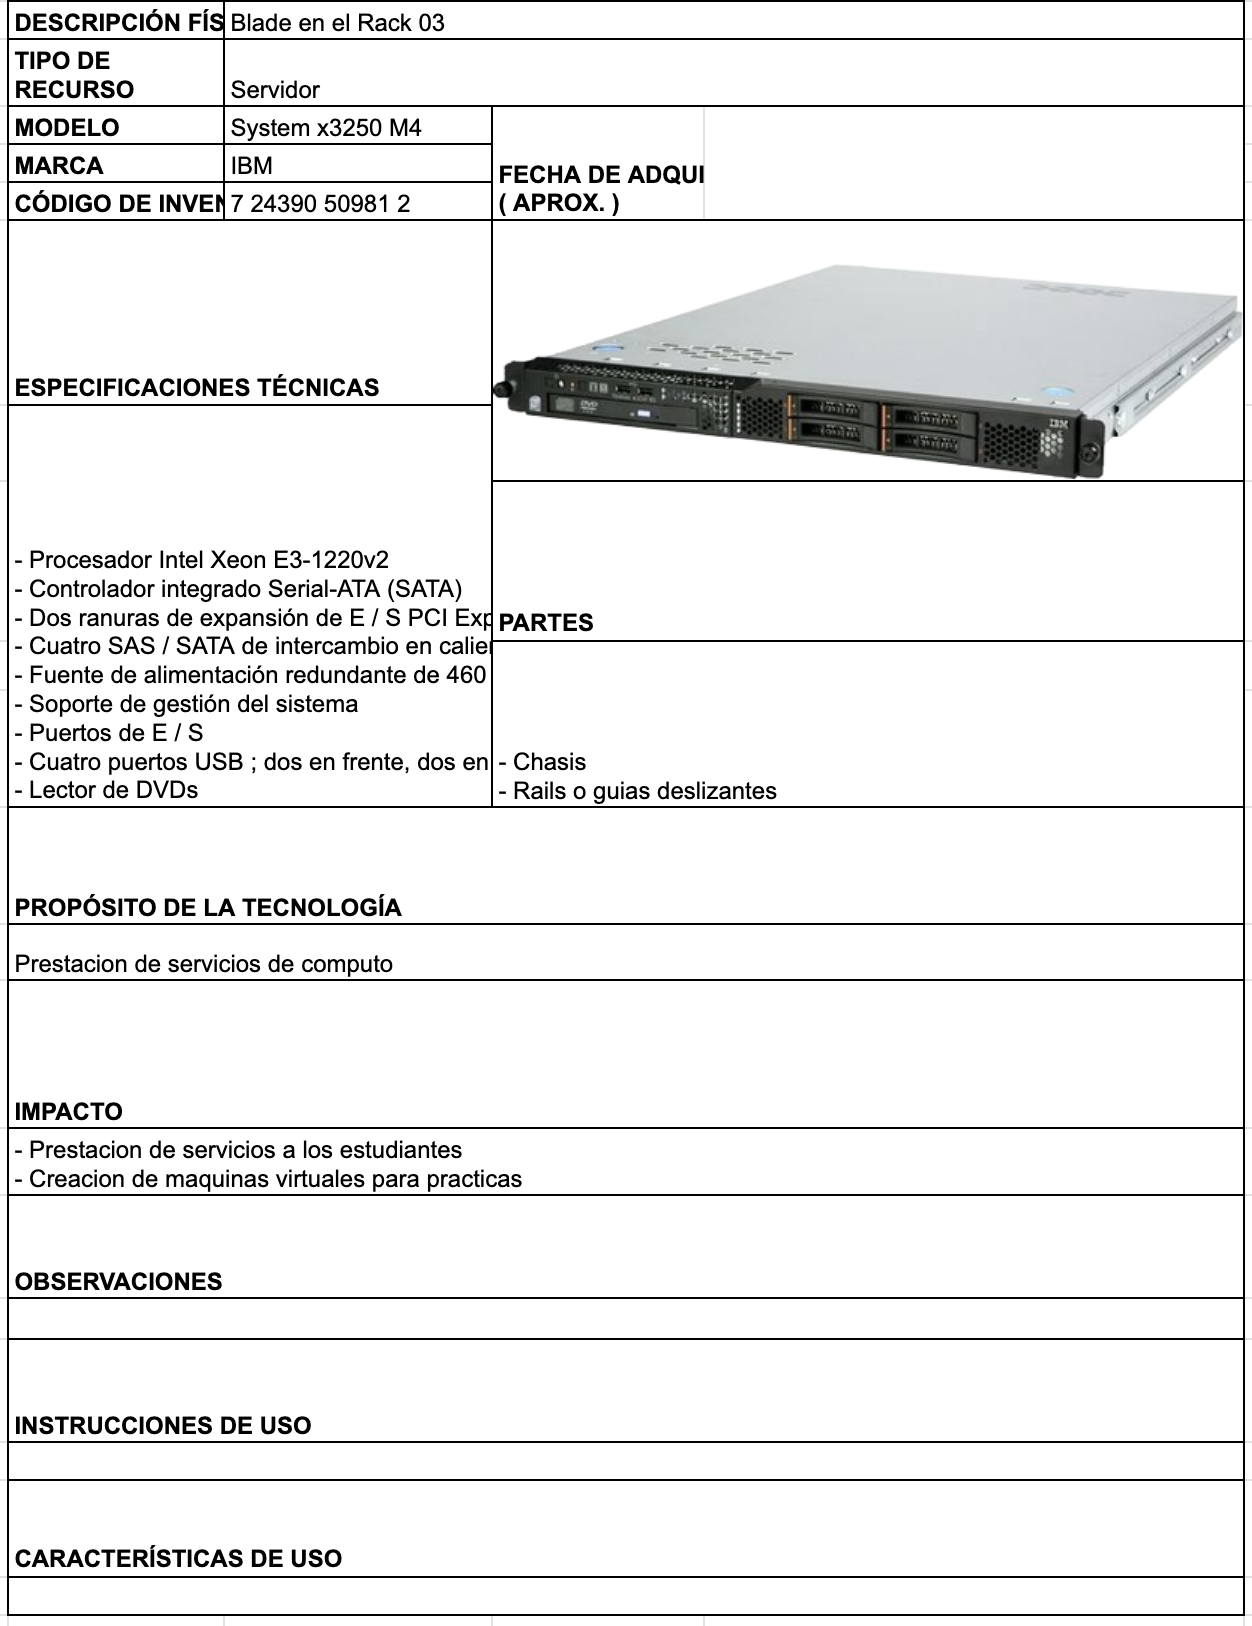
\includegraphics[width=0.18\textwidth,keepaspectratio]{tablas-images/cp1/racks/rack-1.png}} \\ \cline{1-1}
\textbf{MODELO:} System x3250 M4 & \\ \cline{1-1}
\textbf{MARCA:} IBM & \\ \cline{1-1}
\textbf{CÓDIGO DE INVENTARIO:} 7 24390 50980 & \\ \cline{1-1}
\textbf{NUMERO EN CPD:} 53 & \\ \hline
\multicolumn{2}{|l|}{\textbf{ESPECIFICACIONES TÉCNICAS}} \\ \hline
\multicolumn{2}{|p{0.7\textwidth}|}{
- Procesador Intel Xeon E3-1220v2
- Controlador SATA integrado
- 2 ranuras PCI Express
- 4 SAS/SATA intercambio en caliente
- Fuente redundante 460W
- Gestión del sistema
- 4 puertos USB (2 frontal, 2 trasero)
- Lector DVD
} \\ \hline
\multicolumn{2}{|l|}{\textbf{PROPÓSITO:} Prestación de servicios de cómputo} \\ \hline
\multicolumn{2}{|p{0.7\textwidth}|}{\textbf{IMPACTO:} 
- Servicios a estudiantes
- Máquinas virtuales para prácticas} \\ \hline
\multicolumn{2}{|p{0.7\textwidth}|}{\textbf{OBSERVACIONES:} Ninguna} \\ \hline
\end{tabular}
\end{table}

% Rack 4
\begin{table}[H]
\centering
\scriptsize
\setlength{\tabcolsep}{2pt}
\renewcommand{\arraystretch}{1.0}
\caption{Ficha técnica --- Rack 4}
\label{tab:rack-4}
\begin{tabular}{|p{0.5\textwidth}|p{0.2\textwidth}|}
\hline
\multicolumn{2}{|l|}{\textbf{DESCRIPCIÓN FÍSICA:} Servidor tipo rack} \\ \hline
\textbf{TIPO DE RECURSO:} Servidor & 
\multirow{5}{*}{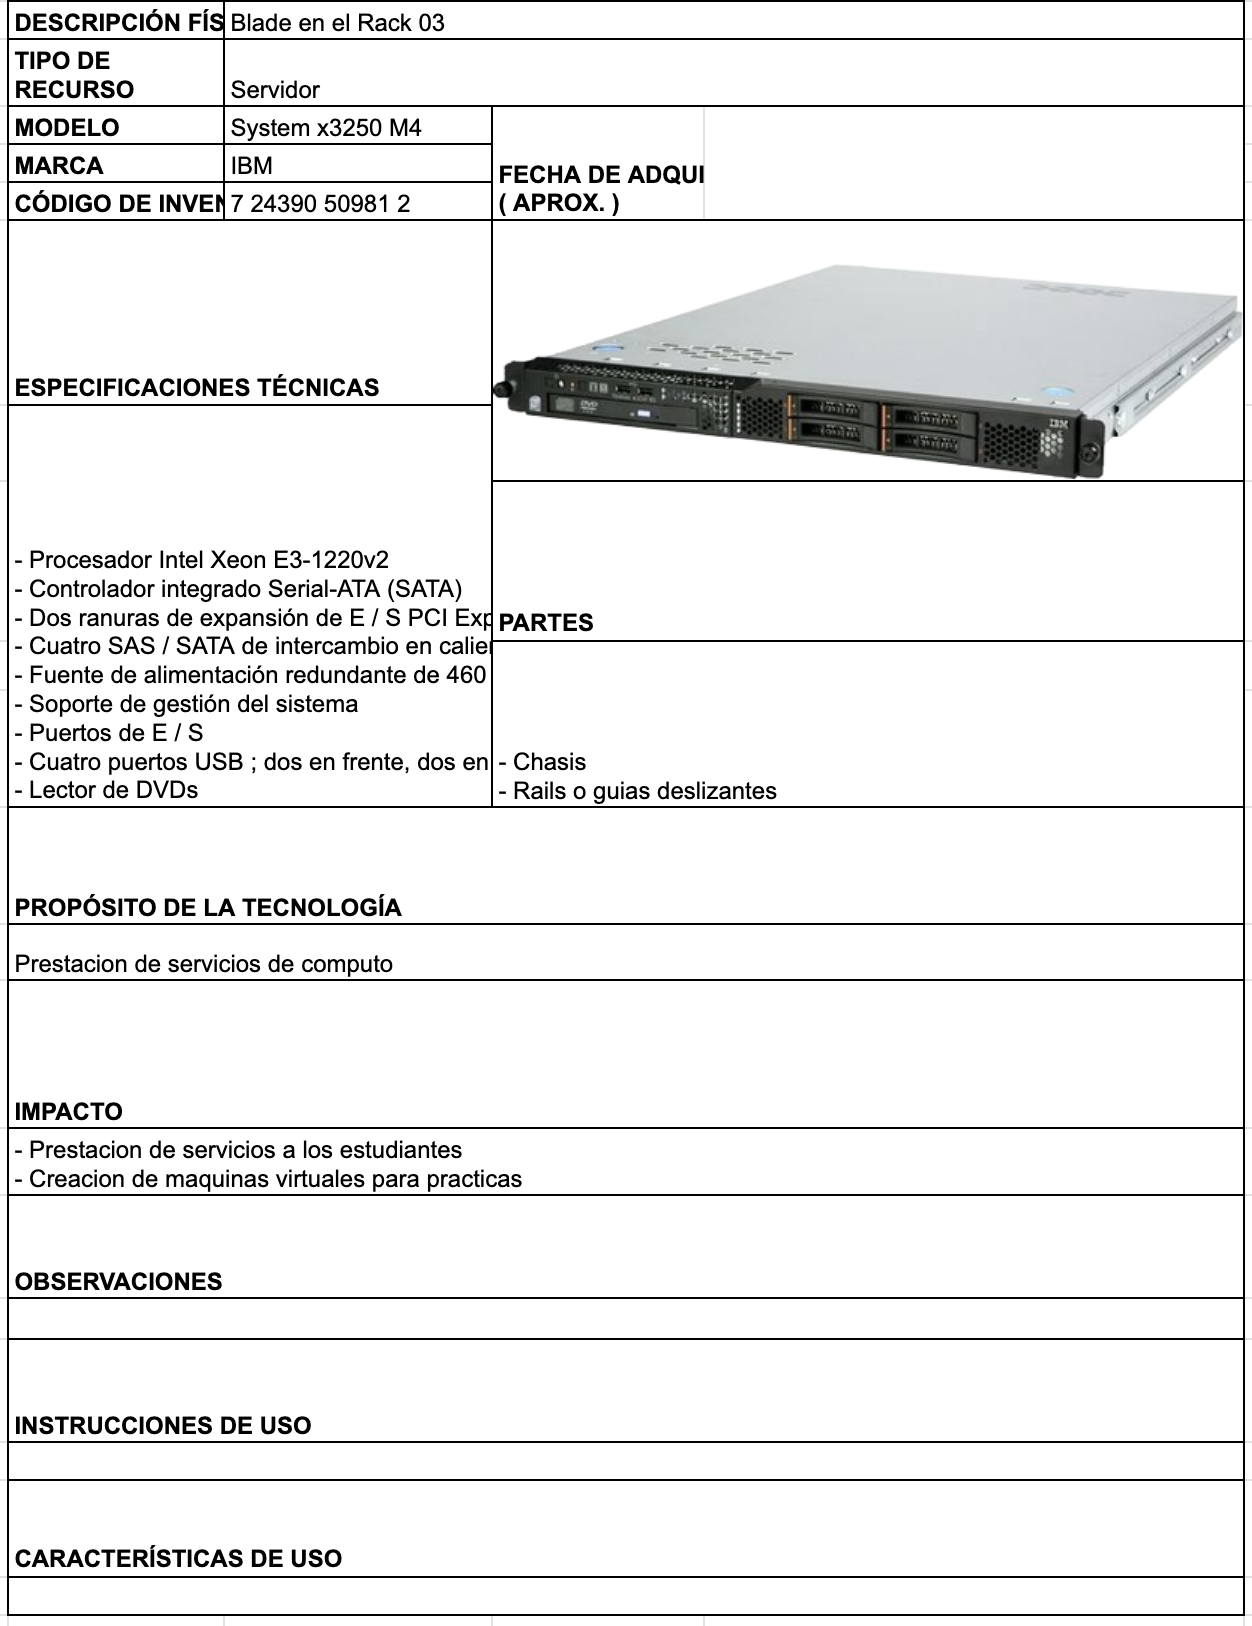
\includegraphics[width=0.18\textwidth,keepaspectratio]{tablas-images/cp1/racks/rack-1.png}} \\ \cline{1-1}
\textbf{MODELO:} System x3250 M4 & \\ \cline{1-1}
\textbf{MARCA:} IBM & \\ \cline{1-1}
\textbf{CÓDIGO DE INVENTARIO:} 7 24390 48735 & \\ \cline{1-1}
\textbf{NUMERO EN CPD:} 52 & \\ \hline
\multicolumn{2}{|l|}{\textbf{ESPECIFICACIONES TÉCNICAS}} \\ \hline
\multicolumn{2}{|p{0.7\textwidth}|}{
- Procesador Intel Xeon E3-1220v2
- Controlador SATA integrado
- 2 ranuras PCI Express
- 4 SAS/SATA intercambio en caliente
- Fuente redundante 460W
- Gestión del sistema
- 4 puertos USB (2 frontal, 2 trasero)
- Lector DVD
} \\ \hline
\multicolumn{2}{|l|}{\textbf{PROPÓSITO:} Prestación de servicios de cómputo} \\ \hline
\multicolumn{2}{|p{0.7\textwidth}|}{\textbf{IMPACTO:} 
- Servicios a estudiantes
- Máquinas virtuales para prácticas} \\ \hline
\multicolumn{2}{|p{0.7\textwidth}|}{\textbf{OBSERVACIONES:} Ninguna} \\ \hline
\end{tabular}
\end{table}

% Rack 5
\begin{table}[H]
\centering
\scriptsize
\setlength{\tabcolsep}{2pt}
\renewcommand{\arraystretch}{1.0}
\caption{Ficha técnica --- Rack 5}\label{tab:rack-5}
\begin{tabular}{|p{0.5\textwidth}|p{0.2\textwidth}|}
\hline
\multicolumn{2}{|l|}{\textbf{DESCRIPCIÓN FÍSICA:} Servidor tipo rack} \\ \hline
\textbf{TIPO DE RECURSO:} Servidor & 
\multirow{5}{*}{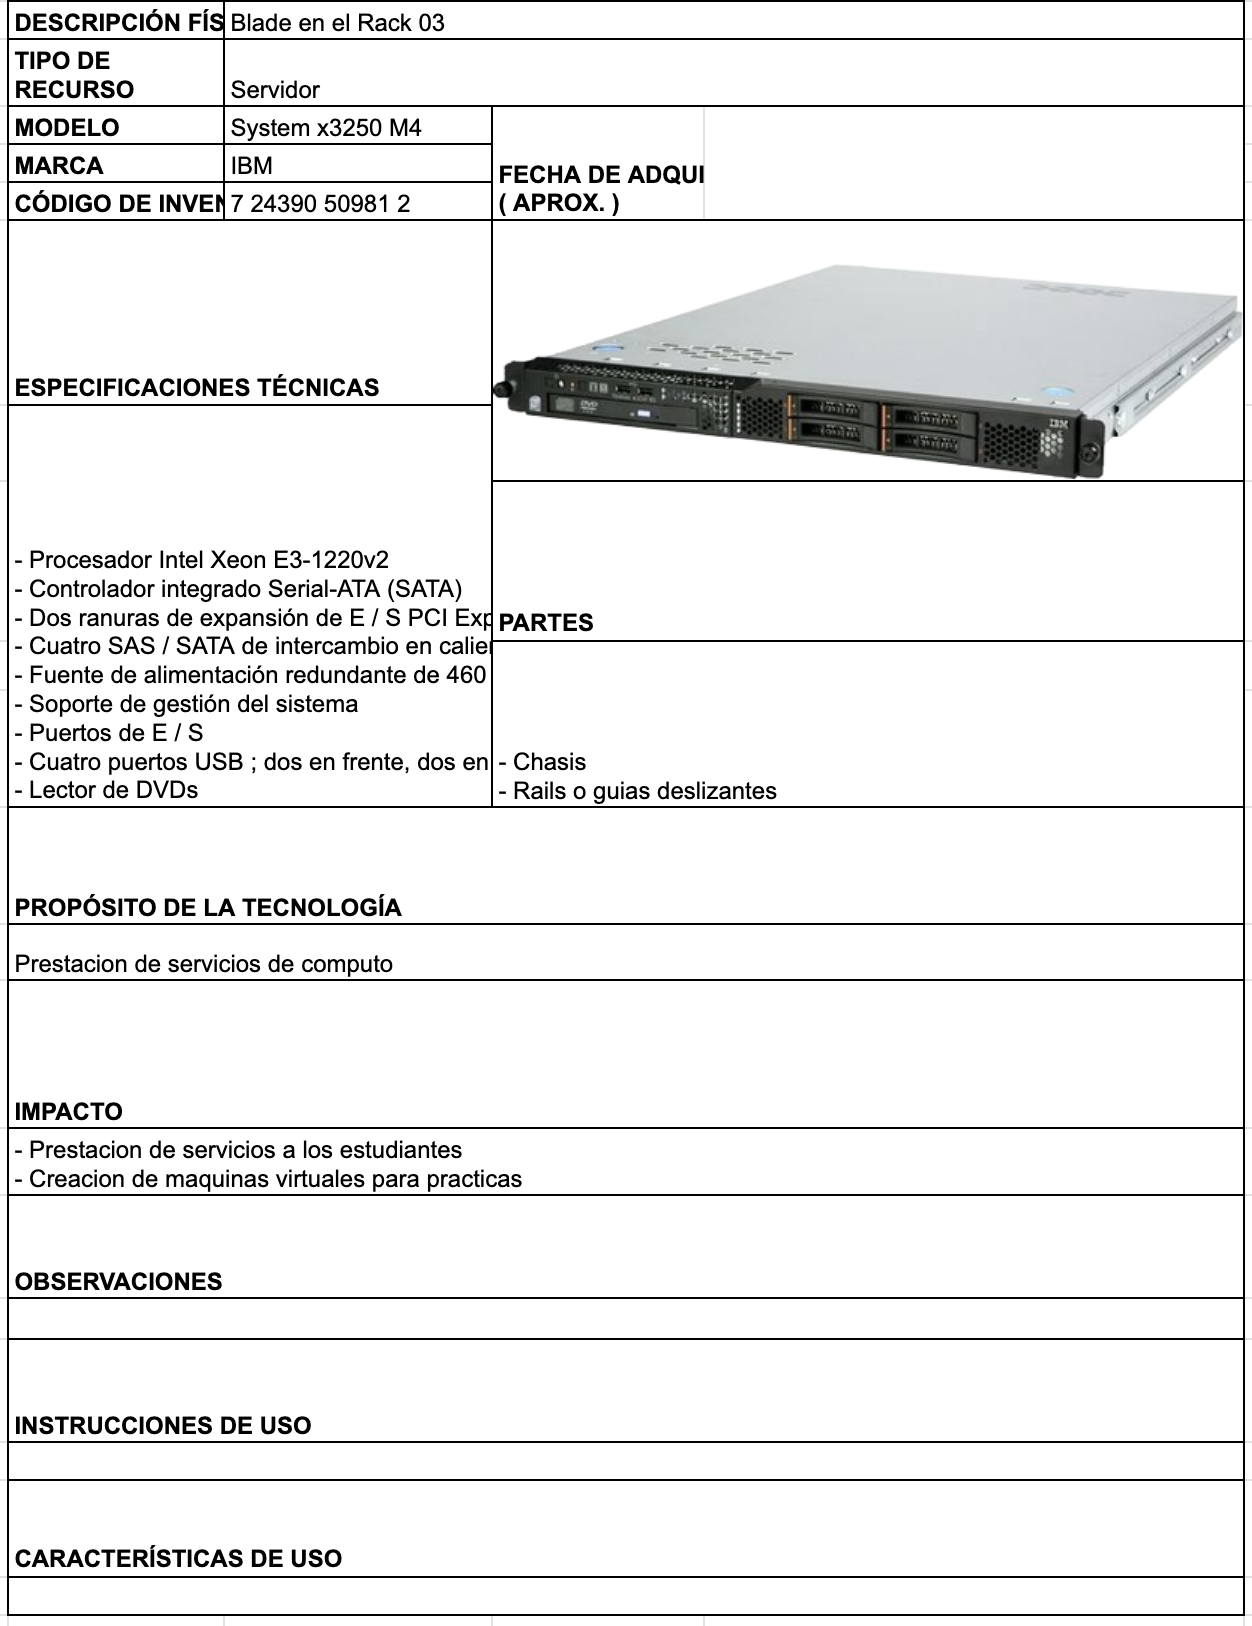
\includegraphics[width=0.18\textwidth,keepaspectratio]{tablas-images/cp1/racks/rack-1.png}} \\ \cline{1-1}
\textbf{MODELO:} System x3250 M4 & \\ \cline{1-1}
\textbf{MARCA:} IBM & \\ \cline{1-1}
\textbf{CÓDIGO DE INVENTARIO:} 51474 & \\ \cline{1-1}
\textbf{NUMERO EN CPD:} 52 & \\ \hline
\multicolumn{2}{|l|}{\textbf{ESPECIFICACIONES TÉCNICAS}} \\ \hline
\multicolumn{2}{|p{0.7\textwidth}|}{
- Procesador Intel Xeon E3-1220v2
- Controlador SATA integrado
- 2 ranuras PCI Express
- 4 SAS/SATA intercambio en caliente
- Fuente redundante 460W
- Gestión del sistema
- 4 puertos USB (2 frontal, 2 trasero)
- Lector DVD
} \\ \hline
\multicolumn{2}{|l|}{\textbf{PROPÓSITO:} Prestación de servicios de cómputo} \\ \hline
\multicolumn{2}{|p{0.7\textwidth}|}{\textbf{IMPACTO:} 
- Servicios a estudiantes
- Máquinas virtuales para prácticas} \\ \hline
\multicolumn{2}{|p{0.7\textwidth}|}{\textbf{OBSERVACIONES:} Ninguna} \\ \hline
\end{tabular}
\end{table}

El cuadro~\ref{tab:nas-1} presenta la ficha técnica del NAS, un sistema de almacenamiento en red modelo TS-832PX-4G de la marca QNAP, el cual se integra como un recurso estratégico en la infraestructura tecnológica. Este dispositivo cuenta con un procesador Annapurna Labs Alpine AL-324 de cuatro núcleos, memoria RAM de 4 GB DDR4 expandible hasta 16 GB, ocho bahías para discos SATA de 3.5 o 2.5 pulgadas, dos puertos de red RJ45 de 2.5 GbE y dos de 10 GbE, además de tres puertos USB 3.2 Gen 1 y ranuras PCIe para expansión. Su consumo energético es de 50.8 W en funcionamiento y 27 W en reposo, lo que permite operación continua. El propósito principal de este NAS es ofrecer almacenamiento compartido y redundante en red, ofreciendo disponibilidad de respaldos y acceso confiable a archivos para proyectos académicos.
% NAS 1
\begin{table}[H]
\centering
\scriptsize
\setlength{\tabcolsep}{2pt}
\renewcommand{\arraystretch}{1.0}
\caption{Ficha técnica --- NAS 1}\label{tab:nas-1}
\begin{tabular}{|p{0.5\textwidth}|p{0.2\textwidth}|}
\hline
\multicolumn{2}{|l|}{\textbf{DESCRIPCIÓN FÍSICA:} Sistema de almacenamiento en red} \\ \hline
\textbf{TIPO DE RECURSO:} NAS & 
\multirow{5}{*}{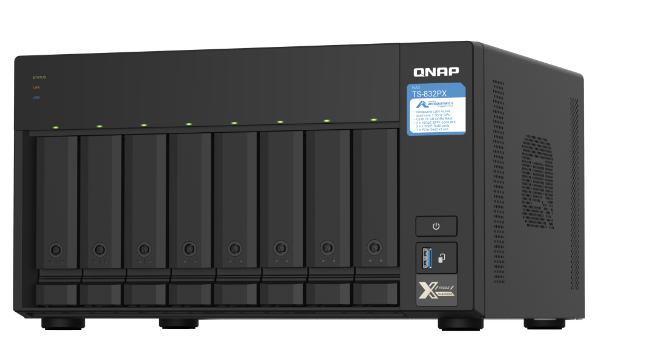
\includegraphics[width=0.18\textwidth,keepaspectratio]{tablas-images/cp1/NAS/nas-1.png}} \\ \cline{1-1}
\textbf{MODELO:} TS-832PX-4G & \\ \cline{1-1}
\textbf{MARCA:} QNAP & \\ \cline{1-1}
\textbf{CÓDIGO DE INVENTARIO:} Por definir & \\ \cline{1-1}
\textbf{FECHA DE ADQUISICIÓN:} & \\ \hline
\multicolumn{2}{|l|}{\textbf{ESPECIFICACIONES TÉCNICAS}} \\ \hline
\multicolumn{2}{|p{0.7\textwidth}|}{
- Procesador: Annapurna Labs Alpine AL-324, 4 núcleos
- RAM: 4 GB DDR4 (exp. a 16 GB)
- Bahías: 8 para discos SATA 3.5"/2.5"
- Puertos Red: 2 x RJ45 2.5GbE, 2 x 10GbE
- Puertos USB: 3 x USB 3.2 Gen 1
- Consumo: 50.8 W (func.), 27 W (reposo)
- Expansión: Ranuras PCIe
} \\ \hline
\multicolumn{2}{|p{0.7\textwidth}|}{\textbf{PROPÓSITO:} Almacenamiento compartido y redundante en red} \\ \hline
\multicolumn{2}{|p{0.7\textwidth}|}{\textbf{IMPACTO:} - Sin NAS: no hay backups ni acceso a archivos} \\ \hline
\multicolumn{2}{|p{0.7\textwidth}|}{\textbf{OBSERVACIONES:} Ninguna} \\ \hline
\end{tabular}
\end{table}

El cuadro~\ref{tab:firewall-1} corresponde a la ficha técnica de un firewall implementado en el \CPD, el cual funciona como sistema de seguridad de red. Se trata de un equipo DELL, modelo PowerEdge T100, con código de inventario 7 24390 46288 9 y chasis en formato torre. Sus especificaciones técnicas incluyen un procesador Intel Xeon E3110 de 3 GHz, 4 GB de memoria DDR2 (2 x 2 GB), un disco duro de 1 TB tipo HDD de 3.5 pulgadas, fuente de alimentación de 305 W, unidad óptica DVD-ROM y conectividad Ethernet. Su propósito principal es la seguridad de la red de servidores, evitando accesos no autorizados y protegiendo los recursos computacionales. Actúa como primera barrera de defensa en el ecosistema de virtualización y servicios del grupo, contribuyendo a la integridad de los datos y a la continuidad de los procesos misionales.
% Firewall 1
\begin{table}[H]
\centering
\scriptsize
\setlength{\tabcolsep}{2pt}
\renewcommand{\arraystretch}{1.0}
\caption{Ficha técnica --- Firewall}\label{tab:firewall-1}
\begin{tabular}{|p{0.5\textwidth}|p{0.2\textwidth}|}
\hline
\multicolumn{2}{|l|}{\textbf{DESCRIPCIÓN FÍSICA:} Sistema de seguridad de red} \\ \hline
\textbf{TIPO DE RECURSO:} Firewall & 
\multirow{5}{*}{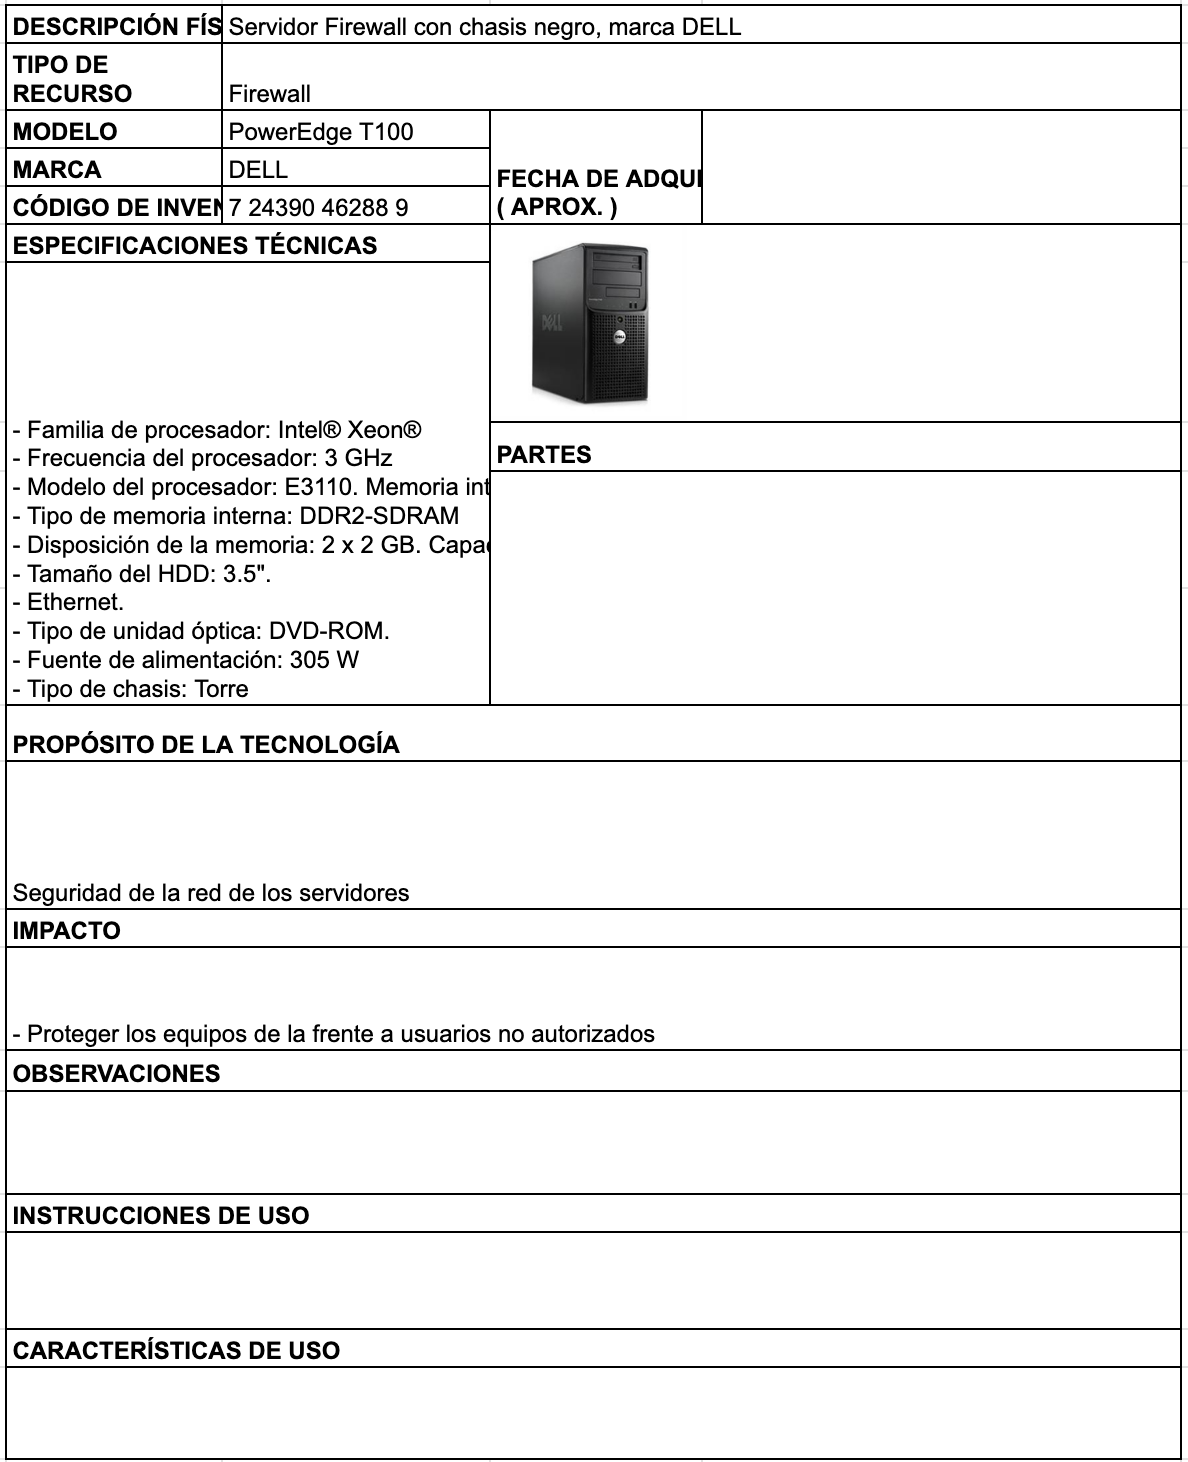
\includegraphics[width=0.18\textwidth,keepaspectratio]{tablas-images/cp1/firewall/firewall.png}} \\ \cline{1-1}
\textbf{MODELO:} PowerEdge T100 & \\ \cline{1-1}
\textbf{MARCA:} DELL & \\ \cline{1-1}
\textbf{CÓDIGO DE INVENTARIO:} 7 24390 46288 9 & \\ \cline{1-1}
\textbf{NÚMERO EN CPF:} No especificado & \\ \hline
\multicolumn{2}{|l|}{\textbf{ESPECIFICACIONES TÉCNICAS}} \\ \hline
\multicolumn{2}{|p{0.7\textwidth}|}{
- Procesador: Intel Xeon E3110 3 GHz
- Memoria: 4 GB DDR2 (2 x 2 GB)
- Almacenamiento: 1 TB HDD 3.5"
- Fuente alimentación: 305 W
- Unidad óptica: DVD-ROM
- Tipo chasis: Torre
- Ethernet
} \\ \hline
\multicolumn{2}{|l|}{\textbf{PROPÓSITO:} Seguridad de la red de servidores} \\ \hline
\multicolumn{2}{|p{0.7\textwidth}|}{\textbf{IMPACTO:} - Protege equipos de usuarios no autorizados} \\ \hline
\multicolumn{2}{|p{0.7\textwidth}|}{\textbf{OBSERVACIONES:} Ninguna} \\ \hline
\end{tabular}
\end{table}